\chapter{Модуль ядра}
\textbf{Цель:} Сборка модуля ядра, работа с device tree.

\vspace{5mm}
\textbf{Полезные ссылки:}
\begin{itemize}
	\item \href{https://linux-kernel-labs.github.io/refs/heads/master/labs/device_drivers.html}{Linux Kernel Labs: Character device drivers}.
	\item \href{https://www.digi.com/resources/examples-guides/use-device-tree-overlays-to-patch-your-device-tree}{DiGi: Use Device Tree Overlays to Patch Your Device Tree}.
\end{itemize}

\vspace{5mm}
\textbf{Описание:}Для начала нужно понять, что в ОС Linux выделяется два пространства: пространство ядра (Kernel Space) и пользовательское пространство (User Space).

Эти два пространства разделены между собой, и взаимодействие может происходить только при помощи специального системного интерфейса (System Call Interface).

\begin{center}
	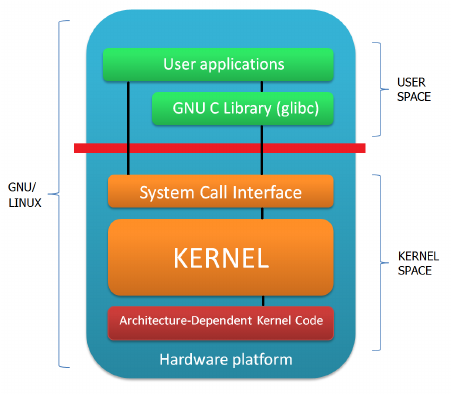
\includegraphics[width=\textwidth]{pic_12}
\end{center}

В пространстве ядра работает, как не удивительно, само ядро ОС, а так же его модули (которые могут быть встроены в основное ядро, или могут быть представлены файлами в rootfs с расширением ko).

Пользовательские приложения и библиотеки работают в пользовательском пространстве. 

Ядро ОС Linux умеет работать с подгружаемыми модулями (если эта опция была активирована при сборке ядра). В качестве отдельных модулей могут выступать как определённые сервисы, предоставляемые ядром, так и драйверы устройств.

В Linux выделяют три типа устройств:
\begin{itemize}
	\item символьное устройство — представлено в файловой системой, минимальный объём данных один символ (или байт), примеры: клавиатура, мышь, принтер, тачскрин, экран, камера, spi устройство, i2c устройство и т.д. 
	\item блочное устройство — представлено в файловой системе, минимальный объём это блок данных, работа ведётся путём монтирования устройства. Примеры: карты памяти, SD карты и пр.  
	\item пакетное устройство — не представлено в файловой системе, устройство для взаимодействия пакетами, примеры: сетевой интерфейс, Wi-Fi, Bluetooth и т.д. 
\end{itemize}

В данной работе, мы создадим шаблон для символьного устройства, с которым можно будет взаимодействовать через пользовательское приложение.

\section{}Сборка модуля

\subsection{}Откройте консоль комбинацией клавиш Ctrl+Alt+T

\subsection{}Создайте рабочий каталог
\begin{lstlisting}[style=bash]
# mkdir -p $BAGET/lab_03 
\end{lstlisting}

\subsection{}Скопируйте в него рабочие файлы
\begin{lstlisting}[style=bash]
# cp -r $BAGET/support/mychar $BAGET/lab_03/
\end{lstlisting}

\subsection{}Перейдите в рабочий каталог и запустите vscode
\begin{lstlisting}[style=bash]
# cd $BAGET/lab_03/mychar; code .
\end{lstlisting}

\textbf{Замечание:} При первом входе, Вас могут спросить, доверяете ли вы автору, нужно нажать на кнопку Yes,  

\begin{center}
	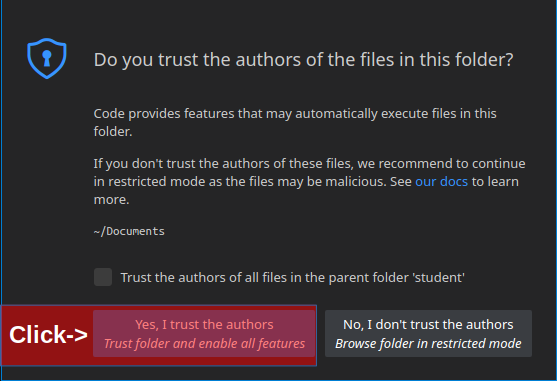
\includegraphics[width=\textwidth]{pic_13}
\end{center}

\subsection{}Добавим путей для разрешения части include директив. Откройте .vscode -> c\_cpp\_properties.json
\begin{center}
	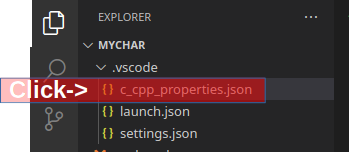
\includegraphics[width=\textwidth]{pic_14}
\end{center}

\subsection{}Допишите в поле includePath следующие строки:\\
\begin{center}
	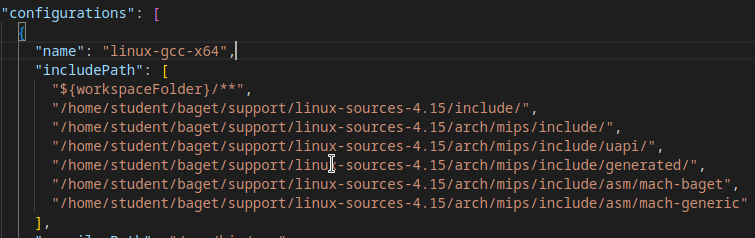
\includegraphics[width=\textwidth]{pic_15}
\end{center}
для удобства, воспользуйтесь файлом vscode\_lines.md в папке support.

Ctrl+S для сохранения

\subsection{}Откройте Makefile. Разберём основные моменты

obj-m  - тут мы задаём имя объектного файла верхнего уровня (файла из которого по итогу будет собран модуль). 

chardev-y — описываем, из каких объектных файлов будет собираться итоговый. 

KERNEL\_SRC — тут мы создаём переменную, которая будет хранить путь к заголовочным файлам ядра.

SRC — в этой переменной мы записываем путь к исходникам модуля, через вызов утилиты pwd. Таким образом, можно рабочую папку переносить куда угодно, без ручных правок. При сборке модуля, текущий путь меняется на путь KERNEL\_SRC, поэтому путь к исходникам модуля ядра должен быть абослютным.

all: — список команд выполняемых при сборке 

clean: — список команд выполняемых при очистке

\subsection{}Посмотрите на содержимое файла mychar\_init.c. Разберём основные моменты

В данном файле содержится минимальный набор кода, необходимый для сборки модуля ядра, и для его функционирования в системе. Нужно помнить, что данный код выполняется в пространстве ядра (Kernel space), соответственно не все парадигмы и функции привычные по работе с приложениями тут будут работать, хотя большинство из них имеют тут аналоги.

Обратите внимание на структур в районе 36 строки. Эта структура считывается ядром, при обращении к модулю, для установления связи между командами, отправляемыми через системный интерфейс, и функциями, которые их будут исполнять. Таким образом, достигается возможность исключить коллизий при работе с группой различных ядер. По той же причини, все структуры и функции объявлены с ключевым словом static.

Следующий момент, это структура объявляемая со строки 25. Параметр .compatible используется ядром, при сканировании дерева устройств. И при наличии совпадения, автоматически загружает модуль ядра.  


\subsection{}Посмотрите на содержимое файла mychar\_dev.c. В этом фале описан процесс инициализации символьного устройства, а так же работа с основными операциями (открытие файла, закрытие файла, считывание и запись данных).
Обратите внимание на функции работы с данными (srisa\_pdrv\_read и srisa\_pdrv\_write), для обмена данными между user space и kernel space используются специальные функции copy\_to\_user и copy\_from\_user.

\subsection{}Если кликать мышкой на вызываемую функцию, при зажатой клавише Ctrl, то редактор откроет вам реализацию этой функции в отдельной вкладке (если реализация находиться в другом файле). Попробуйте, так как далее Вам этот функционал понадобиться, при выполнении самостоятельных работ.

\subsection{}Перейдём в терминал (можно открыть вкладку TERMINAL в vscode, если её не видно, выберите в меню Terminal -> New Terminal) и соберём модуль командой
\begin{lstlisting}[style=bash]
# ARCH=mips CROSS_COMPILE=mips64el-linux-gnuabi64- make
\end{lstlisting}

\subsection{}Вы должны получить следующий вывод
\begin{center}
	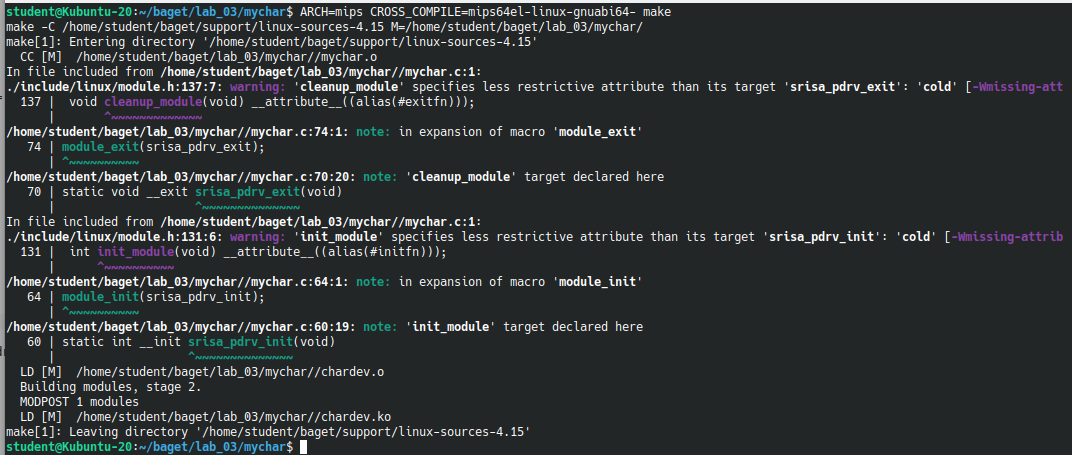
\includegraphics[width=\textwidth]{pic_16}
\end{center}
A в рабочей папке должны появиться несколько файлов, в том числе chardev.ko

\section{Настройка платы}
Для работы с модулями в Linux есть ряд команд

\textbf{insmod <path\_to\_module>} - подключение модуля ядра, с явным указанием пути к файлу, при этом не проверяются зависимости (бывает что один модуль требует предварительного запуска другого модуля).

\textbf{modporbe <module\_name>} - это «умная» версия insmod, проверяет зависимости (файл modules.dep), и подгружает их при необходимости. Не требуется указывать полный путь к модулю, однако модуль должен находиться в папке  /lib/modules/<kernel\_version>/

\textbf{lsmod} — выводит список активированных модулей, с указанием счётчика зависимостей (показывает сколько потоков использует данный модуль)

\textbf{rmmod <module\_name>} - выгрузить указанный модуль (указывается только имя модуля, без расширения ko)

\subsection{}Откройте gtkterm и подключитесь к плате (/dev/ttyUSB1 скорость 115200)

\subsection{}Создадим каталог, для нормальной работы утилиты modporbe. Для этого выполните команду
\begin{lstlisting}[style=bash]
$ mkdir -p /lib/modules/$(uname -r)/
\end{lstlisting}

\subsection{}Создадим два пустых файла
\begin{lstlisting}[style=bash]
$ touch  /lib/modules/$(uname -r)/modules.order
$ touch  /lib/modules/$(uname -r)/modules.builtin
\end{lstlisting}
В данном случае, допустим такой ход, но в общем случае, содержимое этих файлов должно отражать реальность.

\subsection{}Вернёмся в консоль виртуальной машины, и скопируем скомпилированный модуль на плату (проверьте, что плата подключена сетевым шнуром к рабочему ПК)
\begin{lstlisting}[style=bash]
# scp $BAGET/lab_03/mychar/chardev.ko \
netuser@192.168.100.200:/home/netuser/
\end{lstlisting}
пароль - usrnetuser

\subsection{}Вернитесь в терминал платы, и скопируйте ядро
\begin{lstlisting}[style=bash]
$ cp /home/netuser/chardev.ko /lib/modules/$(uname -r)/
\end{lstlisting}

\subsection{}Определим зависимости для модуля, для чего выполните команду 
\begin{lstlisting}[style=bash]
$ depmod
\end{lstlisting}
Данная команда просканирует все модули, в папке /lib/modules/\$(uname -r)/ и запишет о них информацию. После чего модули могут подгружаться командой modprobe. 

\subsection{}Проверим работу нашего модуля, выполнив команду
\begin{lstlisting}[style=bash]
$ modprobe chardev
\end{lstlisting}
Вы должны увидеть надпись 
\begin{lstlisting}[style=stdout]
srisa_pdrv: srisa_pdrv_init
\end{lstlisting}

\subsection{}Просмотрим список загруженных модулей
\begin{lstlisting}[style=bash]
$ lsmod
\end{lstlisting}
Вы должны увидеть надпись 
\begin{lstlisting}[style=stdout]
Module                  Size  Used by
chardev                 4620  0
\end{lstlisting}
Как мы видим, никто не использует наше ядро (Used by равен 0). 

\subsection{}Выполните команду ls /dev/* Обратите внимание, что отсутствует файл srisa\_pdrv, так как он создаётся, только при вызове функции pdrv\_probe, вызываемая только при наличии совместимого периферийного модуля.

\subsection{}Выгрузим из памяти наше ядро
\begin{lstlisting}[style=bash]
$ rmmod chardev
\end{lstlisting}

\section{Правка дерева устройств (device-tree)}
Мы успешно собрали модуль устройства, однако его сейчас никто не использует. Как говорилось выше, часто модули ядра являются драйвером, для взаимодействия с периферией (как внутрипроцессорной, типа интерфейса spi, так и внешней). Для описания взаимодействия между ядром я устройством служит специальная структура дерево устройств (device tree). В ней описывается основная информация о устройстве, а так же могут добавлять параметры, применяемые модулем ядра, при работе с тем или иным устройством. Среди прочего, дерево устройств поддерживает функцию перезаписи, что позволяет создавать мелкие файлы, вносящие исправление в существующее описание, или дополняющее его, в соответствии с требованиями конкретного проекта.

